\subsection{Software Development Methodology}
Software development methodology refers to the practice and process of dividing the project into individual stages and management of tasks required for the completion of the project. There are number of different methodologies used and most famous are Waterfall, Agile, Rapid Application Development (RAD) or DevOps. 

\subsubsection{Project Development Methodology}
Due to the complexity of the project and in order to factor the unknowns the best development methodology for this project would be agile approach. The important characteristics of the agile methodologies are the short iterative cycles, where at the end of each one, a working product is delivered. Short cycles allows for a rapid feedback and will encapsulate all steps required to complete features selected for given iteration \citep{agile1}.

One of the drives for applying agile methodology to this project were expanding requirements. Not all the requirements have been defined at the beginning of the project. Some of the features, like ALIAS Web Extension, have been introduced at the later stages of the project. Hence, the flexible and adaptive methodology like agile was essential. 

Another important aspect of agile is rapid feedback. At the end of each iteration, feedback is provided in terms of delivered product \citep{agilebook}. In terms of this project, the feedback consisted of the test results of the implemented solution, providing insight into any performance and scalability issues. This in turn allowed for any required changes to be applied in the next iteration. Furthermore, regular feedback from project supervisor, Dr Simon Wells, helped to select the critical functionality of ALIAS and shape the final solution.

Although agile methodology is best applied to small teams, the principles of prioritizing tasks and workload, and short iteration cycles can be applied to projects with single developer. This will be the case with this project. 

\subsubsection{Project Schedule}
This project can initially be divided into 4 categories of tasks
\begin{enumerate}
	\item Research
	\item Writing
	\item Development
	\item Benchmark Testing
\end{enumerate}

Figure \ref{fig:projectSchedule} shows the schedule of the project throughout the year. The figure contains the high-level tasks, such as research, write literature review, etc. However, those tasks have been further split into smaller, more manageable tasks throughout the project.  

\begin{landscape}
	\centering
	\begin{figure}[]
		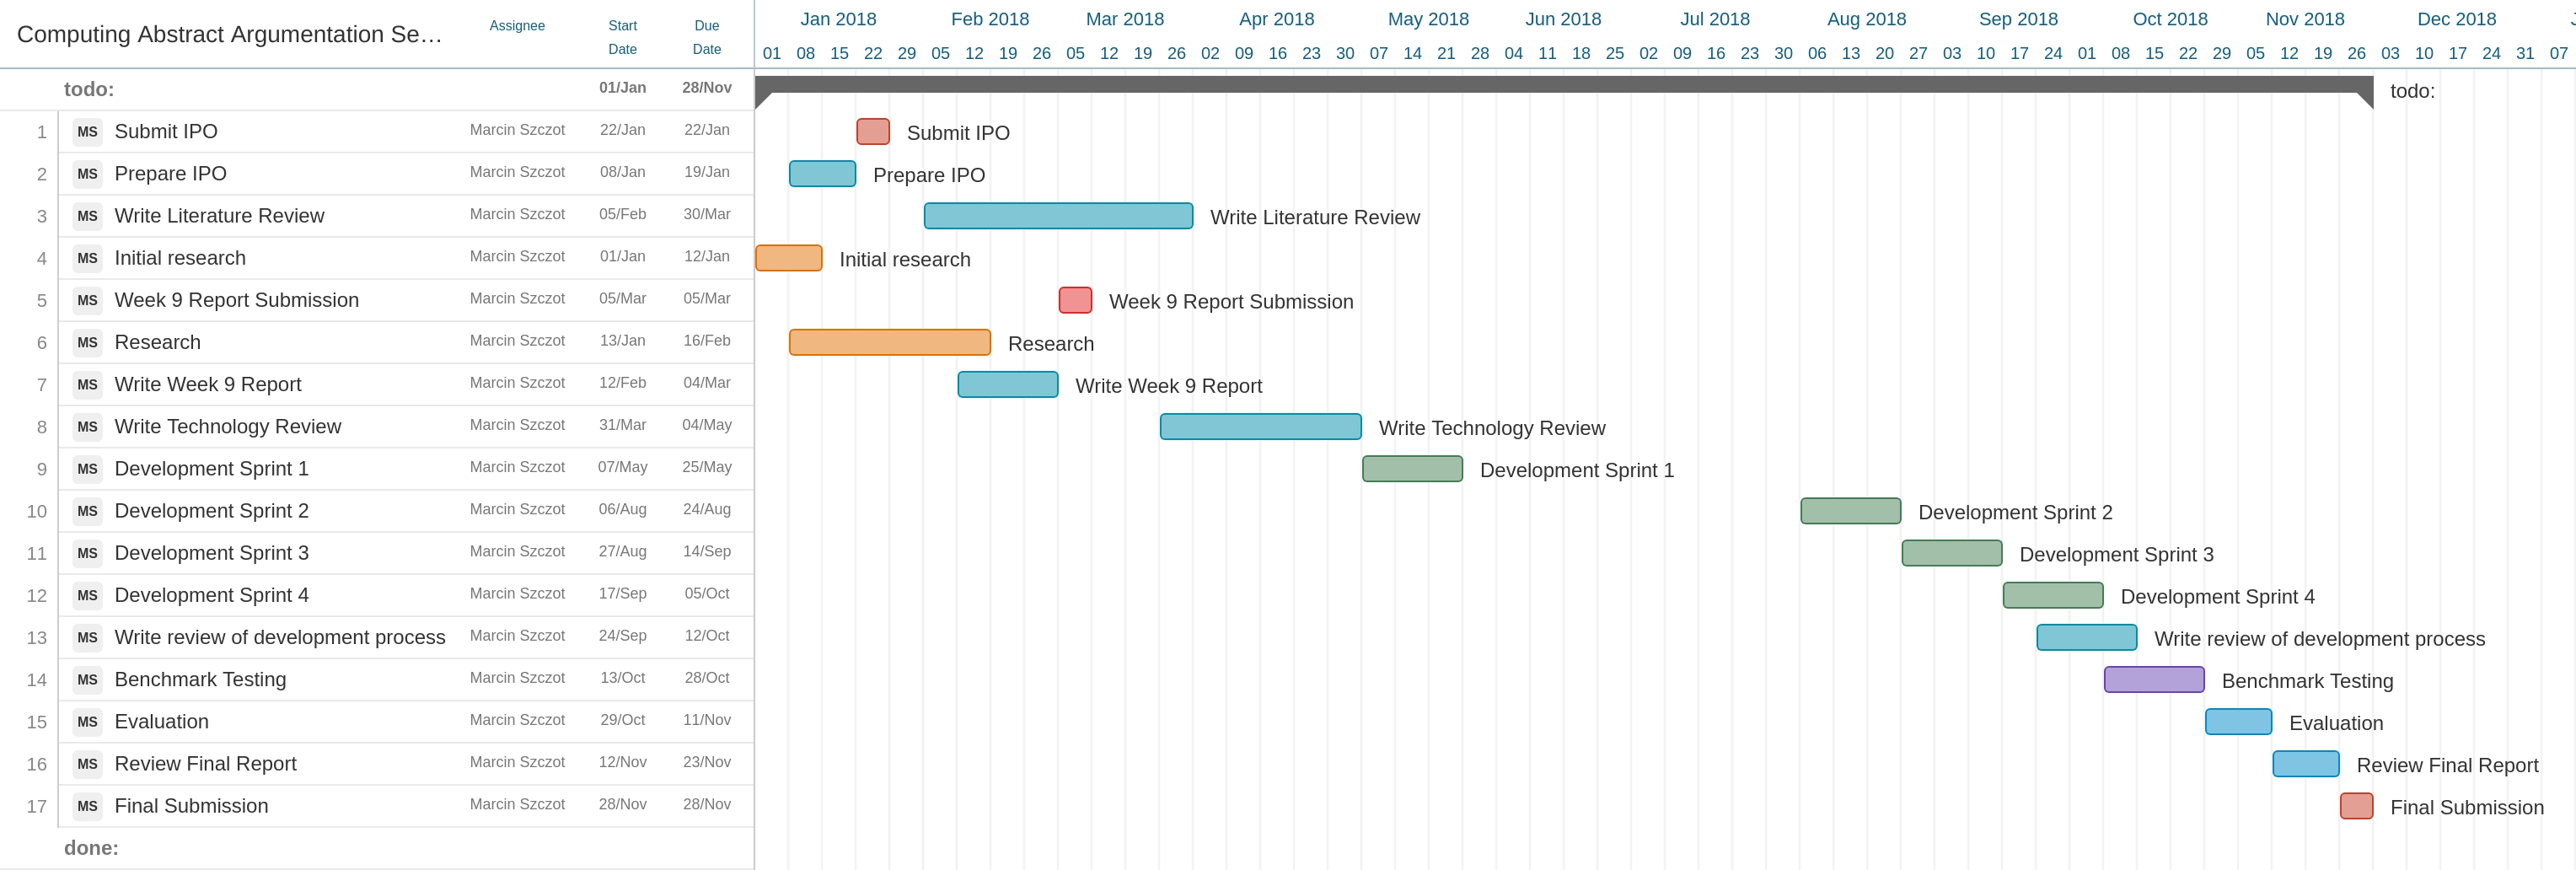
\includegraphics[width=21cm]{gantt}
		\caption{Project Schedule}
		\label{fig:projectSchedule}
	\end{figure}
\end{landscape}

As can bee seen in figure \ref{fig:projectSchedule}, there were 4 development cycles planned. Each development cycle is 3 weeks long and consist of planning session, where number of features to be developed are selected for given iterations, design and development of the solution and testing to verify the application behaves correctly. During the project, the development cycles have also been used to investigate and implement different approaches to computing abstract argumentation semantics.